\documentclass[10pt,twocolumn]{article}
\usepackage[margin=0.7in]{geometry}
\usepackage{booktabs,graphicx,amssymb}
\begin{document}
\begin{table*}[t]
\centering
\caption{RQ1: MAP per clone type on the original query sets (100 queries per type; Table~\ref{tab:rq1rep} repeats the evaluation on 10 replicate query sets; candidates = the query's clones of that type plus methods of other functionalities). Tree kernels on variant D at tuned settings. Mean = mean over the five types. CodeBERT: microsoft/codebert-base, CLS embedding, cosine, first 512 tokens; fine-tuned = contrastive fine-tuning in 5 folds by functionality, each query scored by the model whose training data excluded its functionality. $^{+}$/$^{-}$: significantly better/worse than BM25 (paired bootstrap, 95\%). $^{\uparrow}$/$^{\downarrow}$: tree kernel significantly better/worse than fine-tuned CodeBERT. Best per column in bold.}
\label{tab:rq1}
\small
\begin{tabular}{llcccccc}
\toprule
Method & Setting & T1 & T2 & VST3 & ST3 & MT3 & Mean \\
\midrule
STK & $\lambda$=0.8 & \textbf{1.000} & \textbf{1.000}$^{+}$ & \textbf{1.000}$^{\uparrow}$ & 0.937$^{+}$ & 0.592$^{\downarrow}$ & 0.906 \\
SSTK & $\lambda$=0.1 & \textbf{1.000} & \textbf{1.000}$^{+}$ & \textbf{1.000}$^{\uparrow}$ & 0.939$^{+}$ & 0.606 & 0.909$^{+}$ \\
PTK & $\lambda$=0.4, $\mu$=0.6 & \textbf{1.000} & \textbf{1.000}$^{+}$ & \textbf{1.000}$^{\uparrow}$ & \textbf{0.973}$^{+\uparrow}$ & 0.654 & \textbf{0.926}$^{+}$ \\
\midrule
BM25 & $k_1$=1.2, $b$=0.75 & \textbf{1.000} & 0.969 & 0.989 & 0.854 & 0.630 & 0.888 \\
CodeBERT zs & zero-shot & \textbf{1.000} & 0.992 & 0.981 & 0.882 & 0.485$^{-}$ & 0.868 \\
CodeBERT ft & fine-tuned, 5 folds & \textbf{1.000} & 0.990 & 0.983 & 0.906$^{+}$ & \textbf{0.673} & 0.910$^{+}$ \\
\bottomrule
\end{tabular}
\end{table*}

\begin{figure}[t]\centering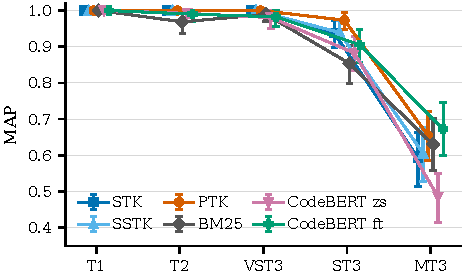
\includegraphics[width=\columnwidth]{figures/rq1_map_by_type}\caption{RQ1: MAP per clone type over 10 replicate query sets (100 queries per type each). Boxes: interquartile range and median; whiskers: min--max.}\label{fig:rq1}\end{figure}
\begin{table*}[t]
\centering
\caption{RQ1 and RQ2 over 10 replicate query sets (seeds 55, 1375, 2084, 2802, 3389, 3501, 6251, 8241, 8828, 9080). Each replicate draws 100 queries per clone type and 100 functional queries at random, independently of the other replicates and of the original sets (Table~\ref{tab:rq1}); tuning queries are excluded. Mean $\pm$ standard deviation over the replicates; MAP per clone type, Mean = mean over the five types, MAP@R for RQ2. Tree kernels on variant D at tuned settings. Best mean per column in bold. $^{+}$/$^{-}$: significantly better/worse than BM25; $^{\uparrow}$/$^{\downarrow}$: tree kernel significantly better/worse than fine-tuned CodeBERT (all distinct queries of the replicates pooled; paired bootstrap over functionalities, 95\%).}
\label{tab:rq1rep}
\footnotesize
\setlength{\tabcolsep}{3.5pt}
\begin{tabular}{lccccccc}
\toprule
 & \multicolumn{6}{c}{RQ1: MAP} & RQ2 \\ \cmidrule(lr){2-7}\cmidrule(lr){8-8}
Method & T1 & T2 & VST3 & ST3 & MT3 & Mean & MAP@R \\
\midrule
STK & \textbf{1.000}$\pm$0.000 & 0.997$\pm$0.005$^{+}$ & \textbf{0.999}$\pm$0.004$^{+\uparrow}$ & 0.959$\pm$0.010$^{+\uparrow}$ & 0.651$\pm$0.040$^{\downarrow}$ & 0.921$\pm$0.008$^{+}$ & 0.248$\pm$0.020$^{-\downarrow}$ \\
SSTK & \textbf{1.000}$\pm$0.000 & 0.999$\pm$0.001$^{+\uparrow}$ & \textbf{0.999}$\pm$0.003$^{+\uparrow}$ & \textbf{0.970}$\pm$0.010$^{+\uparrow}$ & 0.668$\pm$0.041 & 0.927$\pm$0.009$^{+}$ & 0.242$\pm$0.021$^{-\downarrow}$ \\
PTK & \textbf{1.000}$\pm$0.000 & \textbf{1.000}$\pm$0.000$^{+\uparrow}$ & 0.995$\pm$0.006 & 0.969$\pm$0.013$^{+\uparrow}$ & 0.709$\pm$0.034 & \textbf{0.935}$\pm$0.007$^{+}$ & 0.212$\pm$0.022$^{-\downarrow}$ \\
\midrule
BM25 & \textbf{1.000}$\pm$0.000 & 0.972$\pm$0.011 & 0.973$\pm$0.009 & 0.895$\pm$0.022 & 0.657$\pm$0.034 & 0.899$\pm$0.007 & 0.555$\pm$0.021 \\
CodeBERT zs & \textbf{1.000}$\pm$0.000 & 0.982$\pm$0.009 & 0.978$\pm$0.011 & 0.902$\pm$0.014 & 0.579$\pm$0.037 & 0.888$\pm$0.009 & 0.203$\pm$0.014$^{-}$ \\
CodeBERT ft & \textbf{1.000}$\pm$0.000 & 0.988$\pm$0.010 & 0.989$\pm$0.010 & 0.928$\pm$0.014 & \textbf{0.724}$\pm$0.022$^{+}$ & 0.926$\pm$0.006$^{+}$ & \textbf{0.577}$\pm$0.030 \\
\bottomrule
\end{tabular}
\end{table*}

\begin{table*}[t]
\centering
\caption{RQ2: functional similarity on the original query set (100 queries; Table~\ref{tab:rq1rep} gives MAP@R over 10 replicate query sets; relevant = every method of the query's functionality, candidates = the whole corpus). Tree kernels at tuned settings, variant D unless stated. Last two columns: MAP@R by functionality category (pattern: 6 queries, name: 94 queries). CodeBERT: microsoft/codebert-base, CLS embedding, cosine, first 512 tokens; fine-tuned = contrastive fine-tuning in 5 folds by functionality, each query scored by the model whose training data excluded its functionality. $^{+}$/$^{-}$: significantly better/worse than BM25 on MAP@R. $^{\uparrow}$/$^{\downarrow}$: tree kernel significantly better/worse than fine-tuned CodeBERT on MAP@R. }
\label{tab:rq2}
\small
\begin{tabular}{lcccccc}
\toprule
 & & & & & \multicolumn{2}{c}{MAP@R by category} \\ \cmidrule(lr){6-7}
Method & MAP@R & MAP & P@10 & R-Prec & pattern & name \\
\midrule
STK & 0.187$^{-\downarrow}$ & 0.295 & 0.732 & 0.306 & 0.548 & 0.164 \\
SSTK & 0.179$^{-\downarrow}$ & 0.287 & 0.710 & 0.297 & 0.563 & 0.154 \\
PTK & 0.165$^{-\downarrow}$ & 0.269 & 0.689 & 0.276 & \textbf{0.640} & 0.135 \\
SSTK (variant B) & 0.248$^{-\downarrow}$ & 0.373 & 0.750 & 0.363 & 0.555 & 0.229 \\
\midrule
BM25 & 0.477 & 0.616 & 0.803 & \textbf{0.595} & 0.335 & \textbf{0.486} \\
CodeBERT zs & 0.171$^{-}$ & 0.266 & 0.709 & 0.280 & 0.395 & 0.157 \\
CodeBERT ft & \textbf{0.486} & \textbf{0.618} & \textbf{0.815} & 0.587 & 0.568 & 0.481 \\
\bottomrule
\end{tabular}
\end{table*}

\begin{figure}[t]\centering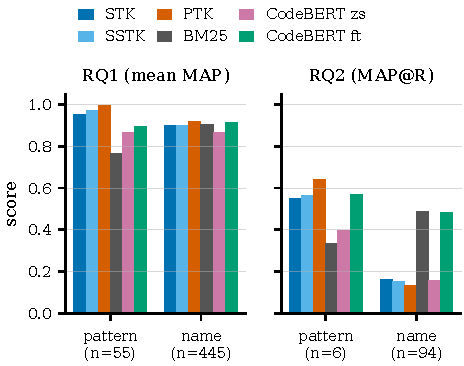
\includegraphics[width=\columnwidth]{figures/rq1_rq2_by_category}\caption{RQ1/RQ2 by functionality category.}\label{fig:cat}\end{figure}
\begin{table*}[t]
\centering
\caption{RQ3: tree variant $\times$ kernel, each at its tuned setting (tuned on 50 separate queries). $\Delta$ tuning = RQ1 mean MAP at the tuned setting minus at KeLP's default ($\lambda$=$\mu$=0.4); $^{*}$: significant (paired bootstrap, 95\%). Best per column in bold.}
\label{tab:rq3}
\small
\begin{tabular}{lllccccc}
\toprule
Variant & Kernel & Setting & ST3 & MT3 & RQ1 mean & RQ2 MAP@R & $\Delta$ tuning \\
\midrule
A & STK & $\lambda$=1.0 & 0.906 & 0.497 & 0.878 & 0.154 & +0.025$^{*}$ \\
 & SSTK & $\lambda$=0.1 & 0.902 & 0.501 & 0.879 & 0.155 & +0.117$^{*}$ \\
 & PTK & $\lambda$=0.6, $\mu$=0.4 & 0.937 & 0.575 & 0.901 & 0.151 & +0.000 \\
\midrule
B & STK & $\lambda$=1.0 & 0.896 & 0.604 & 0.897 & 0.246 & +0.031$^{*}$ \\
 & SSTK & $\lambda$=0.1 & 0.896 & 0.614 & 0.900 & \textbf{0.248} & +0.093$^{*}$ \\
 & PTK & $\lambda$=0.4, $\mu$=0.6 & 0.954 & 0.636 & 0.916 & 0.170 & +0.019$^{*}$ \\
\midrule
C & STK & $\lambda$=0.8 & 0.909 & 0.419 & 0.863 & 0.111 & +0.063$^{*}$ \\
 & SSTK & $\lambda$=0.1 & 0.943 & 0.461 & 0.881 & 0.112 & +0.110$^{*}$ \\
 & PTK & $\lambda$=0.4, $\mu$=0.6 & 0.952 & 0.572 & 0.905 & 0.140 & +0.015$^{*}$ \\
\midrule
D & STK & $\lambda$=0.8 & 0.937 & 0.592 & 0.906 & 0.187 & +0.011$^{*}$ \\
 & SSTK & $\lambda$=0.1 & 0.939 & 0.606 & 0.909 & 0.179 & +0.128$^{*}$ \\
 & PTK & $\lambda$=0.4, $\mu$=0.6 & \textbf{0.973} & \textbf{0.654} & \textbf{0.926} & 0.165 & +0.014$^{*}$ \\
\bottomrule
\end{tabular}
\end{table*}

\begin{figure}[t]\centering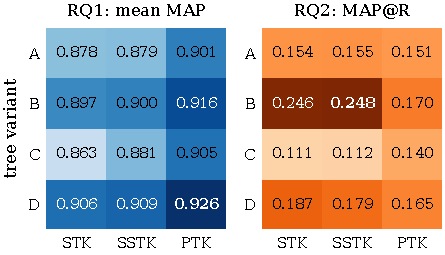
\includegraphics[width=\columnwidth]{figures/rq3_variant_kernel}\caption{RQ3: variant $\times$ kernel.}\label{fig:rq3}\end{figure}
\begin{table}[t]
\centering
\caption{RQ4: fusion of a tree kernel (variant D, tuned) with BM25 or with fine-tuned CodeBERT. Weighted sum = $W\cdot$TK + $(1-W)\cdot$other/max, $W$ tuned on the tuning queries; RRF = reciprocal rank fusion ($k$=60). $^{\dagger}$: significantly better than both components (paired bootstrap, 95\%).}
\label{tab:rq4}
\footnotesize
\setlength{\tabcolsep}{4pt}
\begin{tabular}{lcccc}
\toprule
 & \multicolumn{3}{c}{RQ1 (MAP)} & RQ2 \\ \cmidrule(lr){2-4} \cmidrule(lr){5-5}
Method & ST3 & MT3 & Mean & MAP@R \\
\midrule
\multicolumn{5}{l}{\emph{PTK + BM25, $W$ tuned for RQ1}} \\
\quad PTK & 0.973 & 0.654 & 0.926 & -- \\
\quad BM25 & 0.854 & 0.630 & 0.888 & -- \\
\quad Weighted sum ($W$=0.8) & \textbf{0.978} & \textbf{0.810}$^{\dagger}$ & \textbf{0.957}$^{\dagger}$ & -- \\
\quad RRF & 0.949 & 0.746$^{\dagger}$ & 0.939$^{\dagger}$ & -- \\
\midrule
\multicolumn{5}{l}{\emph{PTK + CodeBERT ft, $W$ tuned for RQ1}} \\
\quad PTK & 0.973 & 0.654 & 0.926 & -- \\
\quad CodeBERT ft & 0.906 & 0.673 & 0.910 & -- \\
\quad Weighted sum ($W$=0.6) & \textbf{0.980} & \textbf{0.796}$^{\dagger}$ & \textbf{0.955}$^{\dagger}$ & -- \\
\quad RRF & 0.976 & 0.763$^{\dagger}$ & 0.947$^{\dagger}$ & -- \\
\midrule
\multicolumn{5}{l}{\emph{STK + BM25, $W$ tuned for RQ2}} \\
\quad STK & -- & -- & -- & 0.187 \\
\quad BM25 & -- & -- & -- & \textbf{0.477} \\
\quad Weighted sum ($W$=0.0) & -- & -- & -- & \textbf{0.477} \\
\quad RRF & -- & -- & -- & 0.336 \\
\midrule
\multicolumn{5}{l}{\emph{STK + CodeBERT ft, $W$ tuned for RQ2}} \\
\quad STK & -- & -- & -- & 0.187 \\
\quad CodeBERT ft & -- & -- & -- & 0.486 \\
\quad Weighted sum ($W$=0.1) & -- & -- & -- & \textbf{0.487} \\
\quad RRF & -- & -- & -- & 0.360 \\
\bottomrule
\end{tabular}
\end{table}

\begin{figure*}[t]\centering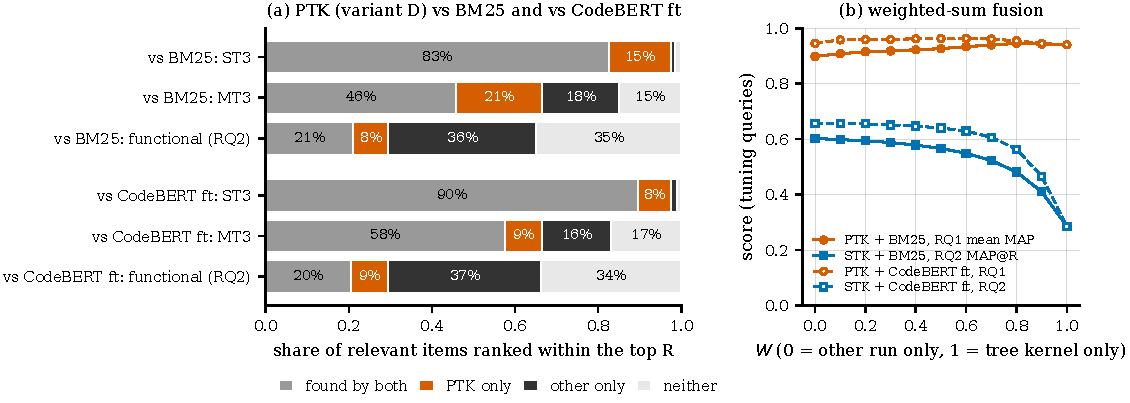
\includegraphics[width=\textwidth]{figures/rq4_complementarity_fusion}\caption{RQ4.}\label{fig:rq4}\end{figure*}
\begin{table*}[t]
\centering
\caption{RQ4 over the 10 replicate query sets (Table~\ref{tab:rq1rep}): fusion of a tree kernel (variant D, tuned) with BM25 or with fine-tuned CodeBERT, at the $W$ tuned on the tuning queries (as in Table~\ref{tab:rq4}). Mean $\pm$ standard deviation over the replicates. $^{\dagger}$: significantly better than both components (all distinct queries of the replicates pooled; paired bootstrap over functionalities, 95\%).}
\label{tab:rq4rep}
\footnotesize
\setlength{\tabcolsep}{4pt}
\begin{tabular}{lcccc}
\toprule
 & \multicolumn{3}{c}{RQ1 (MAP)} & RQ2 \\ \cmidrule(lr){2-4} \cmidrule(lr){5-5}
Method & ST3 & MT3 & Mean & MAP@R \\
\midrule
\multicolumn{5}{l}{\emph{PTK + BM25, $W$ tuned for RQ1}} \\
\quad PTK & 0.969$\pm$0.013 & 0.709$\pm$0.034 & 0.935$\pm$0.007 & -- \\
\quad BM25 & 0.895$\pm$0.022 & 0.657$\pm$0.034 & 0.899$\pm$0.007 & -- \\
\quad Weighted sum ($W$=0.8) & \textbf{0.989}$\pm$0.008$^{\dagger}$ & \textbf{0.849}$\pm$0.031$^{\dagger}$ & \textbf{0.968}$\pm$0.007$^{\dagger}$ & -- \\
\quad RRF & 0.972$\pm$0.012 & 0.777$\pm$0.028 & 0.949$\pm$0.006$^{\dagger}$ & -- \\
\midrule
\multicolumn{5}{l}{\emph{PTK + CodeBERT ft, $W$ tuned for RQ1}} \\
\quad PTK & 0.969$\pm$0.013 & 0.709$\pm$0.034 & 0.935$\pm$0.007 & -- \\
\quad CodeBERT ft & 0.928$\pm$0.014 & 0.724$\pm$0.022 & 0.926$\pm$0.006 & -- \\
\quad Weighted sum ($W$=0.6) & \textbf{0.991}$\pm$0.004$^{\dagger}$ & \textbf{0.860}$\pm$0.025$^{\dagger}$ & \textbf{0.970}$\pm$0.005$^{\dagger}$ & -- \\
\quad RRF & 0.986$\pm$0.008$^{\dagger}$ & 0.821$\pm$0.026$^{\dagger}$ & 0.960$\pm$0.005$^{\dagger}$ & -- \\
\midrule
\multicolumn{5}{l}{\emph{STK + BM25, $W$ tuned for RQ2}} \\
\quad STK & -- & -- & -- & 0.248$\pm$0.020 \\
\quad BM25 & -- & -- & -- & \textbf{0.555}$\pm$0.021 \\
\quad Weighted sum ($W$=0.0) & -- & -- & -- & \textbf{0.555}$\pm$0.021 \\
\quad RRF & -- & -- & -- & 0.409$\pm$0.020 \\
\midrule
\multicolumn{5}{l}{\emph{STK + CodeBERT ft, $W$ tuned for RQ2}} \\
\quad STK & -- & -- & -- & 0.248$\pm$0.020 \\
\quad CodeBERT ft & -- & -- & -- & 0.577$\pm$0.030 \\
\quad Weighted sum ($W$=0.1) & -- & -- & -- & \textbf{0.579}$\pm$0.030 \\
\quad RRF & -- & -- & -- & 0.441$\pm$0.019 \\
\bottomrule
\end{tabular}
\end{table*}

\begin{figure*}[t]\centering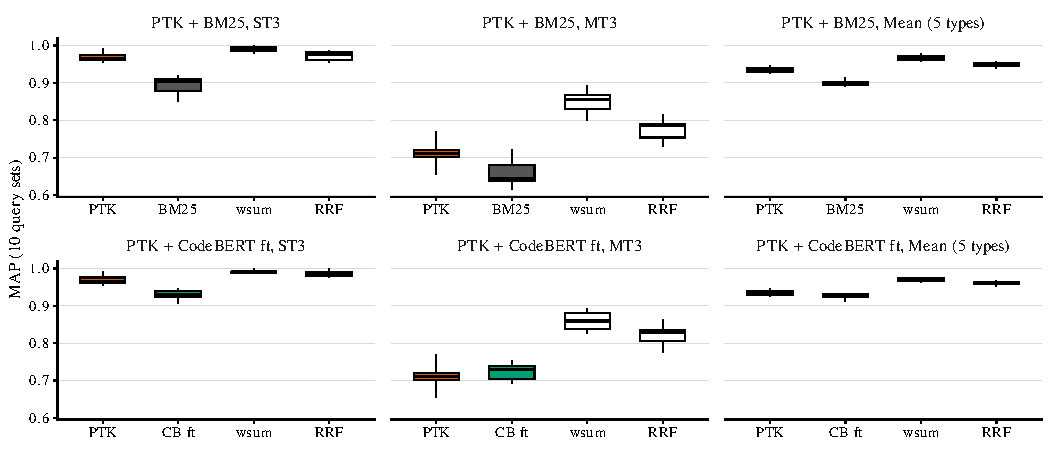
\includegraphics[width=\textwidth]{figures/rq4_fusion_replicates}\caption{RQ4 over 10 replicate query sets: MAP of PTK, the other method and their fusions (weighted sum at the tuned $W$; RRF). Boxes: interquartile range and median; whiskers: min--max.}\label{fig:rq4rep}\end{figure*}
\begin{figure*}[t]\centering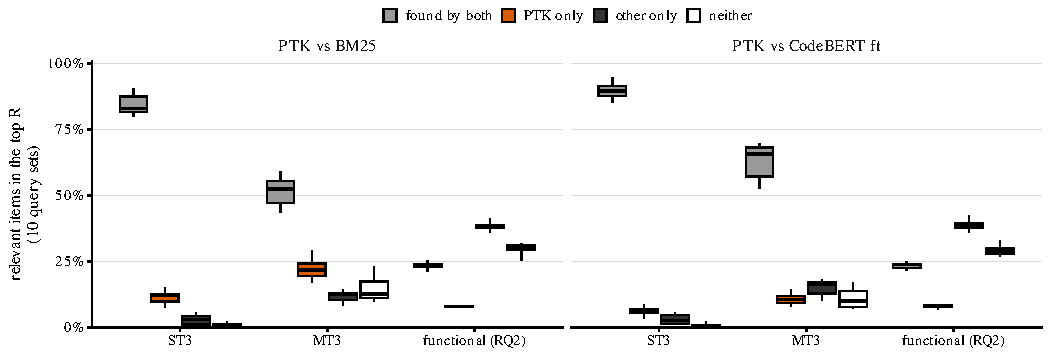
\includegraphics[width=\textwidth]{figures/rq4_complementarity_replicates}\caption{RQ4 complementarity over 10 replicate query sets: share of relevant items ranked within the top R by both, one, or neither of PTK (variant D) and the other method. Boxes: interquartile range and median; whiskers: min--max.}\label{fig:rq4comprep}\end{figure*}
\begin{table*}[t]
\centering
\caption{Robustness: the same queries against a corpus enlarged with 58,103 BigCloneBench false positives (72,782 methods; variant D, tuned). Main = original corpus (14,679 methods). $^{+}$/$^{-}$: significantly better/worse than BM25 on the enlarged corpus. $^{\uparrow}$/$^{\downarrow}$: tree kernel significantly better/worse than fine-tuned CodeBERT on the enlarged corpus. }
\label{tab:e5}
\small
\begin{tabular}{lcccccc}
\toprule
 & \multicolumn{2}{c}{MT3 MAP} & \multicolumn{2}{c}{RQ1 mean MAP} & \multicolumn{2}{c}{RQ2 MAP@R} \\
\cmidrule(lr){2-3} \cmidrule(lr){4-5} \cmidrule(lr){6-7}
Method & Main & Enlarged & Main & Enlarged & Main & Enlarged \\
\midrule
STK & 0.592 & 0.454 & 0.906 & 0.854$^{+\uparrow}$ & 0.187 & 0.089$^{-\downarrow}$ \\
SSTK & 0.606 & 0.483 & 0.909 & 0.866$^{+\uparrow}$ & 0.179 & 0.082$^{-\downarrow}$ \\
PTK & 0.654 & 0.514$^{+}$ & 0.926 & 0.882$^{+\uparrow}$ & 0.165 & 0.078$^{-\downarrow}$ \\
\midrule
BM25 & 0.630 & 0.432 & 0.888 & 0.804 & 0.477 & 0.259 \\
CodeBERT zs & 0.485 & 0.332$^{-}$ & 0.868 & 0.805 & 0.171 & 0.081$^{-}$ \\
CodeBERT ft & 0.673 & 0.475 & 0.910 & 0.831$^{+}$ & 0.486 & 0.249 \\
\bottomrule
\end{tabular}
\end{table*}

\begin{table*}[t]
\centering
\caption{RQ5: cost on one CPU thread (AMD Ryzen 7 8845HS laptop), corpus of 14,679 methods, mean over 20 queries. Preparation = parsing all methods into trees (tree kernels) or tokens and building the index (BM25); set-up = loading the corpus and computing self-similarities; per query = one query scored against the whole corpus. Tree kernels at tuned settings. CodeBERT: preparation = encoding the corpus one method at a time (estimated from 200 methods); set-up = loading the model; per query = encoding the query plus cosine against the stored corpus embeddings; zero-shot and fine-tuned models cost the same at inference. Fine-tuning the five fold models took a further 6.6 h (8 threads).}
\label{tab:rq5}
\small
\begin{tabular}{llrrrr}
\toprule
Variant & Method & Preparation (s) & Set-up (s) & Per query (s) & Per pair ($\mu$s) \\
\midrule
A & STK & 12.6 & 20.8 & 3.65 & 249 \\
 & SSTK &  & 20.5 & 3.68 & 251 \\
 & PTK &  & 51.2 & 14.84 & 1011 \\
\midrule
B & STK & 13.3 & 10.0 & 0.51 & 35 \\
 & SSTK &  & 9.8 & 0.54 & 37 \\
 & PTK &  & 23.4 & 5.68 & 387 \\
\midrule
C & STK & 6.9 & 10.9 & 2.43 & 166 \\
 & SSTK &  & 11.1 & 2.44 & 166 \\
 & PTK &  & 16.2 & 4.13 & 282 \\
\midrule
D & STK & 7.6 & 9.6 & 1.46 & 99 \\
 & SSTK &  & 9.9 & 1.50 & 102 \\
 & PTK &  & 15.7 & 3.40 & 232 \\
\midrule
-- & BM25 & 5.1 & -- & 0.12 & 8 \\
-- & CodeBERT & 6190 & 3.3 & 0.37 & 25 \\
\bottomrule
\end{tabular}
\end{table*}

\begin{figure}[t]\centering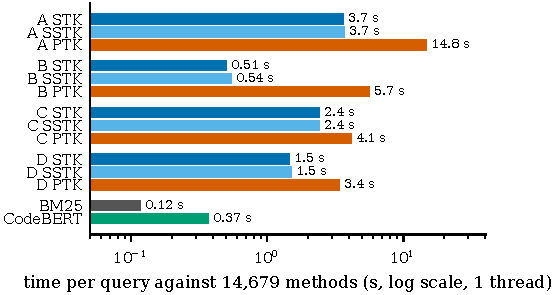
\includegraphics[width=\columnwidth]{figures/rq5_time_per_query}\caption{RQ5: time per query.}\label{fig:rq5}\end{figure}
\begin{figure}[t]\centering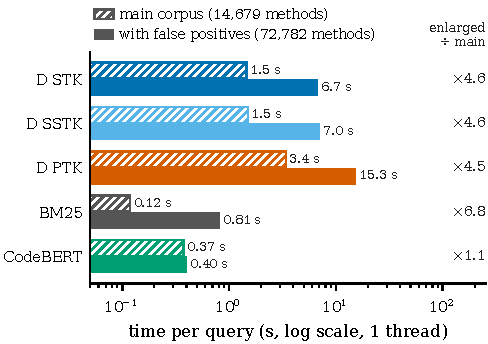
\includegraphics[width=\columnwidth]{figures/rq5_time_e5}\caption{RQ5: time per query, main vs enlarged corpus.}\label{fig:rq5e5}\end{figure}
\end{document}
